\documentclass{beamer}\usepackage[]{graphicx}\usepackage[]{color}
%% maxwidth is the original width if it is less than linewidth
%% otherwise use linewidth (to make sure the graphics do not exceed the margin)
\makeatletter
\def\maxwidth{ %
  \ifdim\Gin@nat@width>\linewidth
    \linewidth
  \else
    \Gin@nat@width
  \fi
}
\makeatother

\definecolor{fgcolor}{rgb}{0.345, 0.345, 0.345}
\newcommand{\hlnum}[1]{\textcolor[rgb]{0.686,0.059,0.569}{#1}}%
\newcommand{\hlstr}[1]{\textcolor[rgb]{0.192,0.494,0.8}{#1}}%
\newcommand{\hlcom}[1]{\textcolor[rgb]{0.678,0.584,0.686}{\textit{#1}}}%
\newcommand{\hlopt}[1]{\textcolor[rgb]{0,0,0}{#1}}%
\newcommand{\hlstd}[1]{\textcolor[rgb]{0.345,0.345,0.345}{#1}}%
\newcommand{\hlkwa}[1]{\textcolor[rgb]{0.161,0.373,0.58}{\textbf{#1}}}%
\newcommand{\hlkwb}[1]{\textcolor[rgb]{0.69,0.353,0.396}{#1}}%
\newcommand{\hlkwc}[1]{\textcolor[rgb]{0.333,0.667,0.333}{#1}}%
\newcommand{\hlkwd}[1]{\textcolor[rgb]{0.737,0.353,0.396}{\textbf{#1}}}%

\usepackage{framed}
\makeatletter
\newenvironment{kframe}{%
 \def\at@end@of@kframe{}%
 \ifinner\ifhmode%
  \def\at@end@of@kframe{\end{minipage}}%
  \begin{minipage}{\columnwidth}%
 \fi\fi%
 \def\FrameCommand##1{\hskip\@totalleftmargin \hskip-\fboxsep
 \colorbox{shadecolor}{##1}\hskip-\fboxsep
     % There is no \\@totalrightmargin, so:
     \hskip-\linewidth \hskip-\@totalleftmargin \hskip\columnwidth}%
 \MakeFramed {\advance\hsize-\width
   \@totalleftmargin\z@ \linewidth\hsize
   \@setminipage}}%
 {\par\unskip\endMakeFramed%
 \at@end@of@kframe}
\makeatother

\definecolor{shadecolor}{rgb}{.97, .97, .97}
\definecolor{messagecolor}{rgb}{0, 0, 0}
\definecolor{warningcolor}{rgb}{1, 0, 1}
\definecolor{errorcolor}{rgb}{1, 0, 0}
\newenvironment{knitrout}{}{} % an empty environment to be redefined in TeX

\usepackage{alltt}
\usepackage{graphicx}
\usepackage{epstopdf}

\newcommand\myheading[1]{%
  \par\bigskip
  {\Large\bfseries#1}\par\smallskip}
\IfFileExists{upquote.sty}{\usepackage{upquote}}{}

\begin{document}

\title{Functions and packages}
\author{David Matten}
\date{30 April 2014}

\maketitle

\begin{frame}[fragile]{Overview}




\begin{itemize}

\item Heirachy
\item What is a function?
\item Built in and Write your own
\item What about packages?
\item Built in and Write your own
\item How to install and load packages
\end{itemize}

\end{frame}


\begin{frame}[fragile]{Heirachy}

\begin{figure}[ht!]
\centering
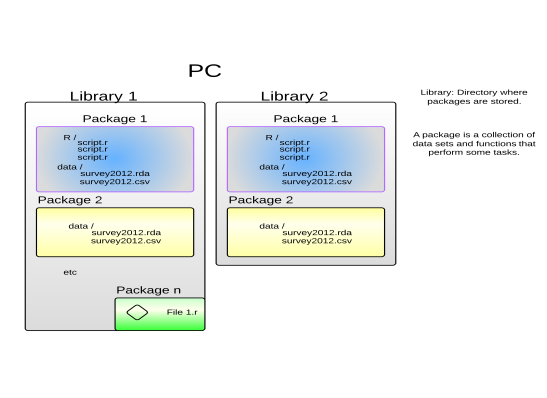
\includegraphics[width=90mm]{pictures/heirachy.jpg}
\label{overflow}
\end{figure}

\end{frame}


\begin{frame}[fragile]{.libPaths()}
\begin{knitrout}
\definecolor{shadecolor}{rgb}{0.969, 0.969, 0.969}\color{fgcolor}\begin{kframe}
\begin{alltt}
\hlkwd{.libPaths}\hlstd{()}
\end{alltt}
\begin{verbatim}
## [1] "/home/dave/R/x86_64-pc-linux-gnu-library/3.1"
## [2] "/usr/local/lib/R/site-library"               
## [3] "/usr/lib/R/site-library"                     
## [4] "/usr/lib/R/library"
\end{verbatim}
\end{kframe}
\end{knitrout}

\end{frame}


\begin{frame}[fragile]{What is a function?}
\begin{itemize}
\item A function is a piece of code that performs a task.
\item We have seen the use of c() already. And a few other functions (maybe you didn’t know they were functions).
\end{itemize}
An example
Imagine we had some predicted values, actual values and we want to calculate the root, mean, square error (RMSE) between them.
\end{frame}


\begin{frame}[fragile]{}
\begin{knitrout}
\definecolor{shadecolor}{rgb}{0.969, 0.969, 0.969}\color{fgcolor}\begin{kframe}
\begin{alltt}
\hlstd{actual} \hlkwb{<-} \hlkwd{c}\hlstd{(}\hlnum{1}\hlstd{,} \hlnum{5}\hlstd{,} \hlnum{10}\hlstd{,} \hlnum{20}\hlstd{)}
\hlstd{predicted} \hlkwb{<-} \hlkwd{c}\hlstd{(}\hlnum{1.1}\hlstd{,} \hlnum{4.8}\hlstd{,} \hlnum{10.5}\hlstd{,} \hlnum{18.6}\hlstd{)}
\hlkwd{sqrt}\hlstd{(}\hlkwd{mean}\hlstd{((actual} \hlopt{-} \hlstd{predicted)}\hlopt{^}\hlnum{2}\hlstd{))}
\end{alltt}
\begin{verbatim}
## [1] 0.7517
\end{verbatim}
\begin{alltt}
\hlstd{calcRMSE} \hlkwb{<-} \hlkwa{function}\hlstd{(}\hlkwc{a}\hlstd{,} \hlkwc{b}\hlstd{) \{}
    \hlkwd{sqrt}\hlstd{(}\hlkwd{mean}\hlstd{((a} \hlopt{-} \hlstd{b)}\hlopt{^}\hlnum{2}\hlstd{))}
\hlstd{\}}

\hlkwd{calcRMSE}\hlstd{(actual, predicted)}
\end{alltt}
\begin{verbatim}
## [1] 0.7517
\end{verbatim}
\end{kframe}
\end{knitrout}

\end{frame}


\begin{frame}
Not only is it cumbersome to write out the full contents of a function every time you want to do whatever calculation, but also it can become very difficult to quickly see what it does. %\vspace{\baselineskip}
Look at the next few pieces of code for increasing complex examples, can you tell what each does from the code?
\end{frame}


\begin{frame}[fragile]{sd}
\begin{figure}[ht!]
\centering
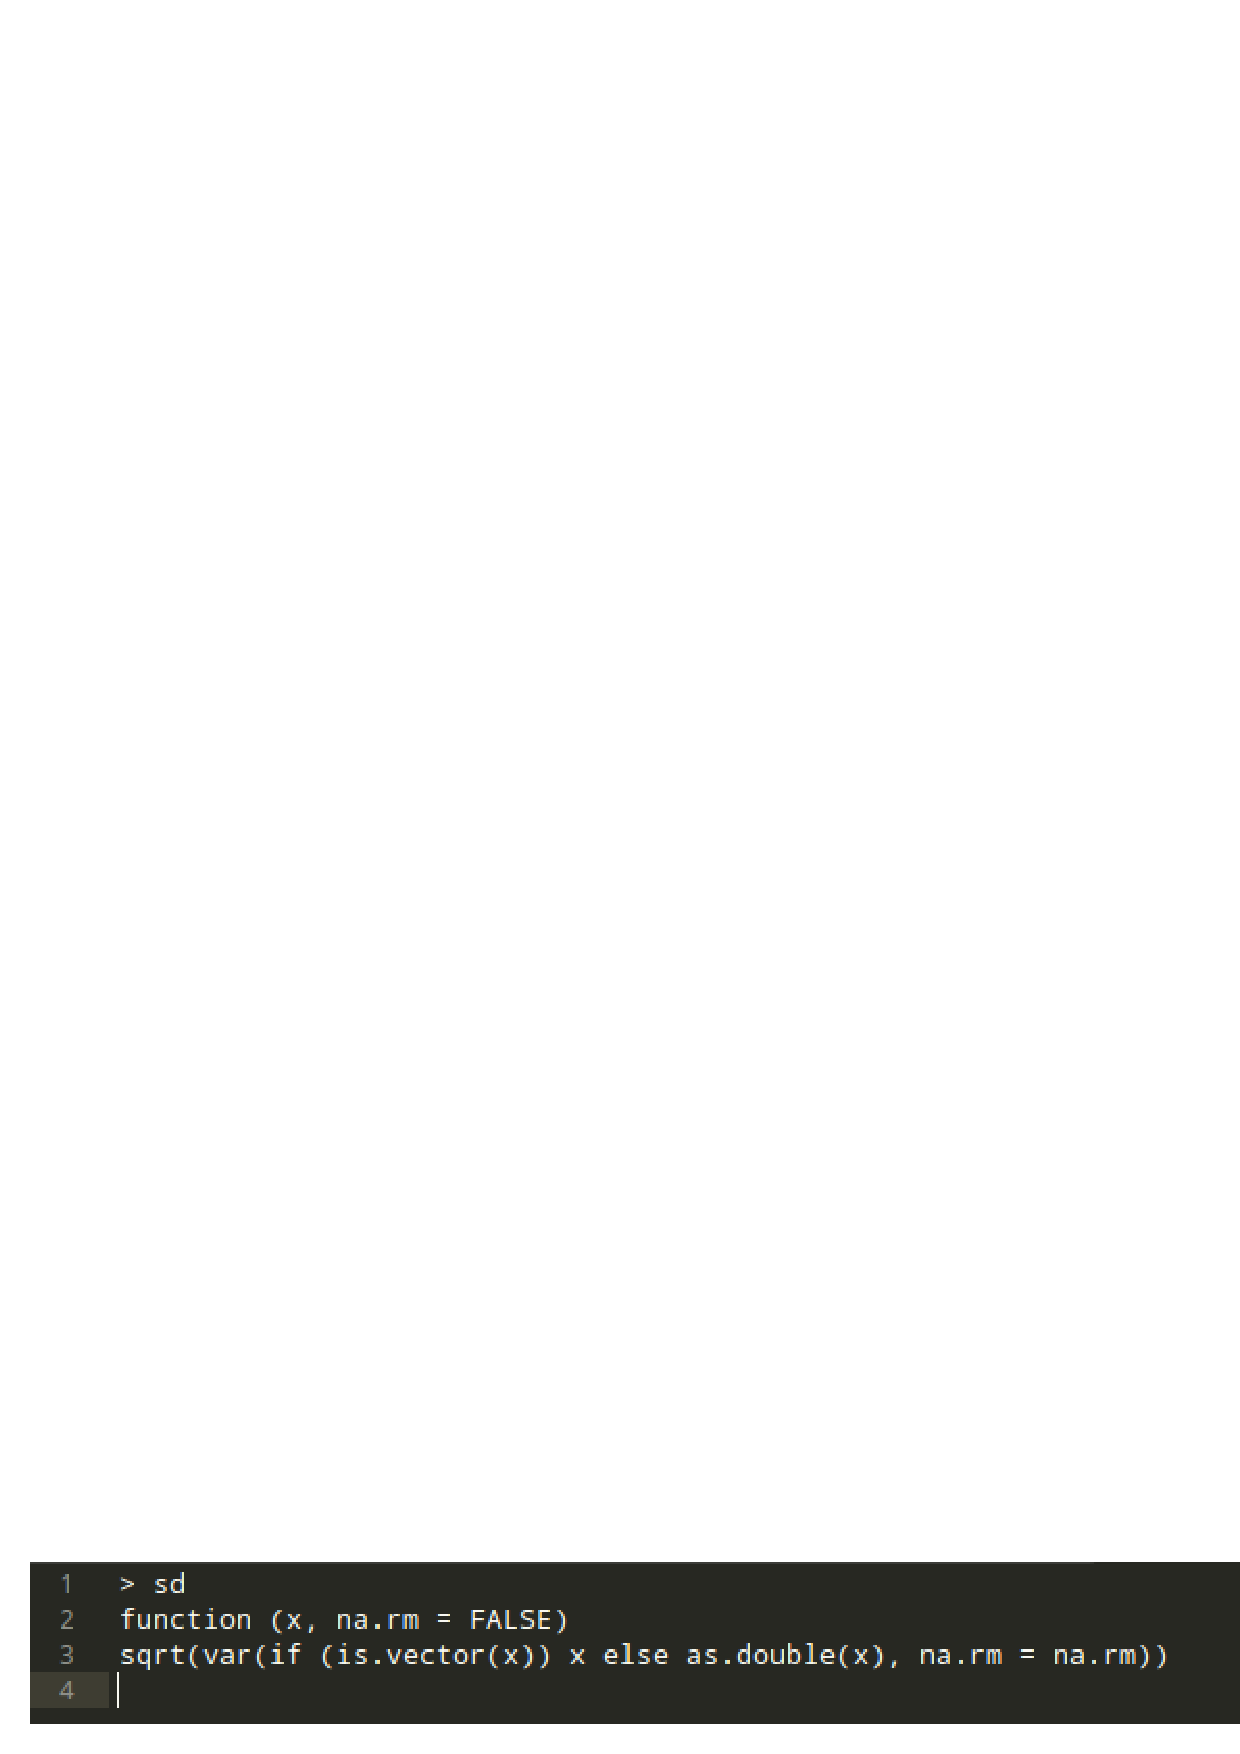
\includegraphics[width=90mm]{pictures/sd.jpg}
\label{overflow}
\end{figure}
\end{frame}


\begin{frame}[fragile]{factor}
\begin{figure}[ht!]
\centering
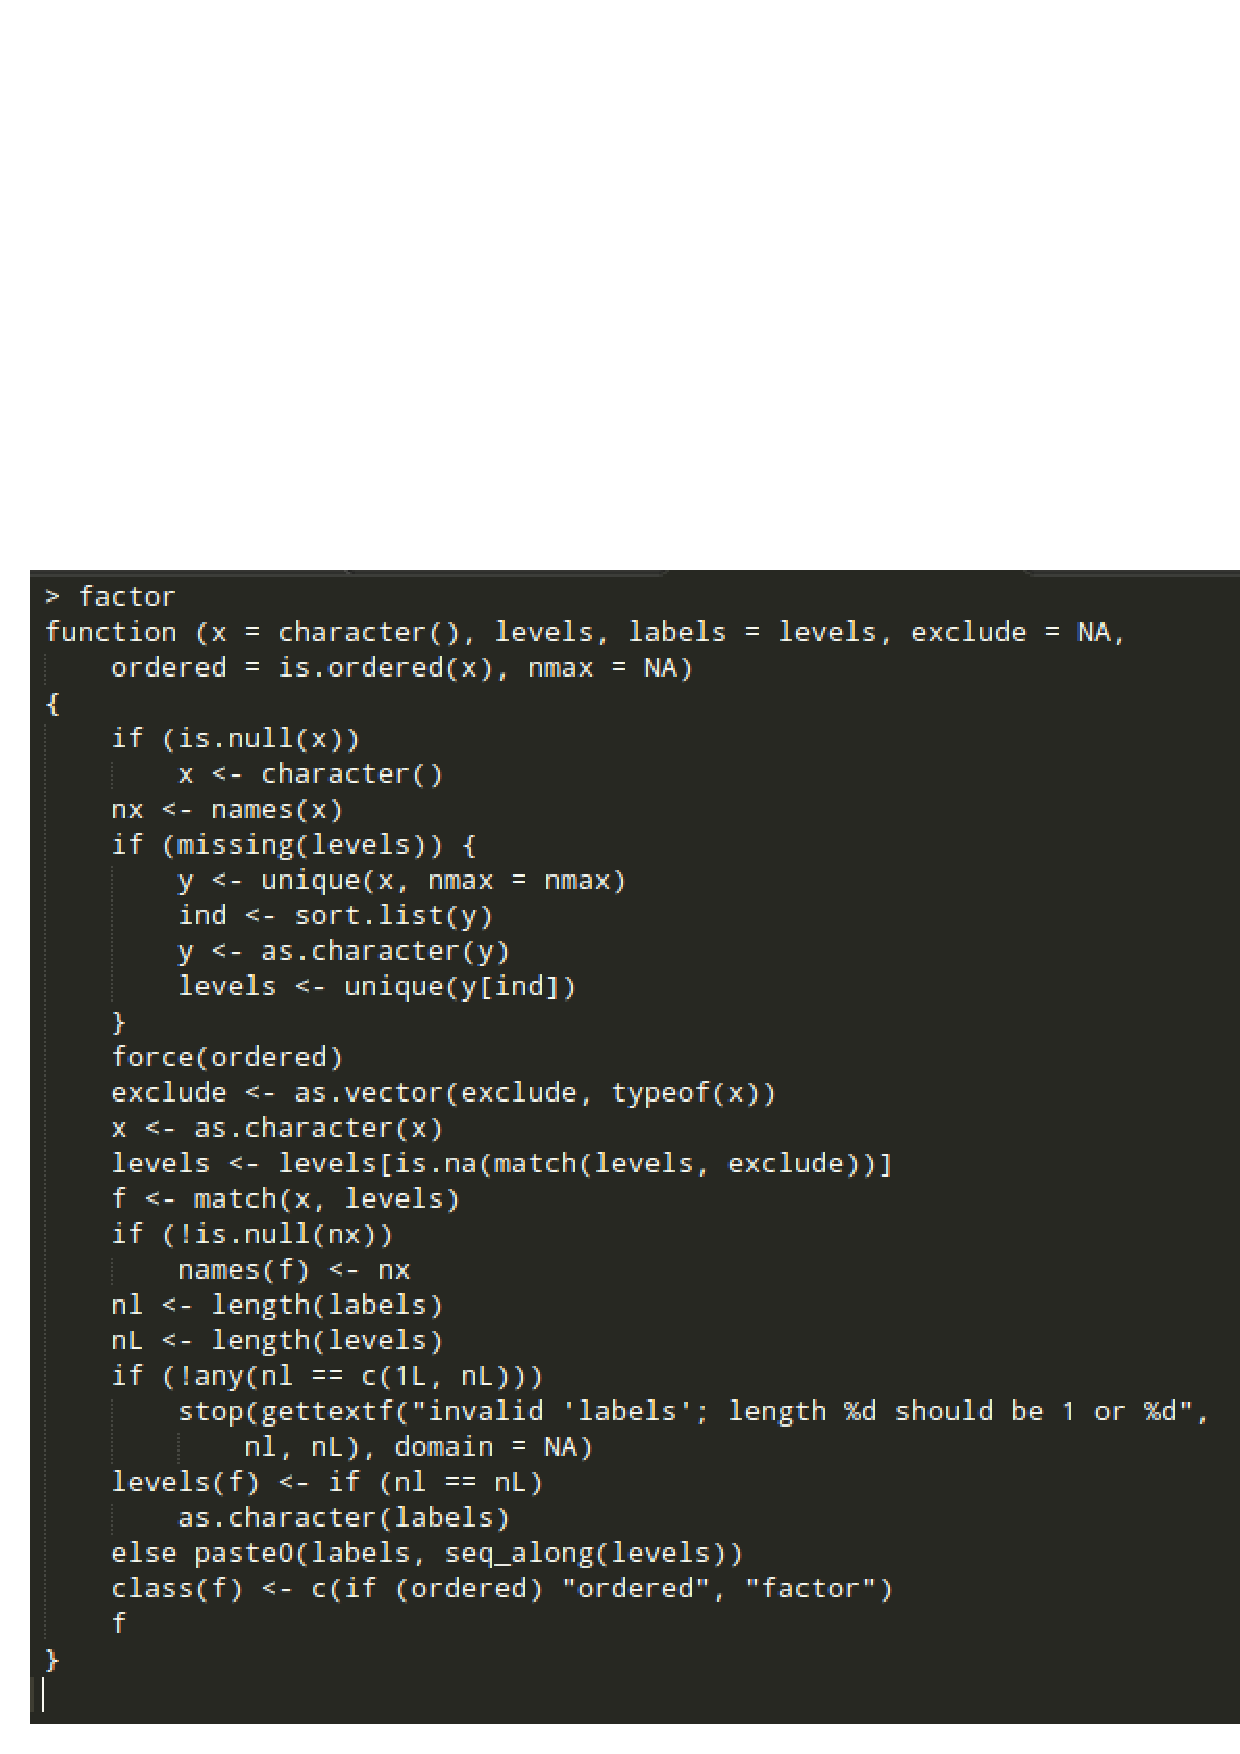
\includegraphics[width=90mm]{pictures/factor.jpg}
\label{overflow}
\end{figure}
\end{frame}


\begin{frame}[fragile]{table}
\begin{figure}[ht!]
\centering

\includegraphics[width=90mm]{pictures/table.jpg}
\label{overflow}
\end{figure}
\end{frame}


\begin{frame}[fragile]{How to install and load packages}
rawr
\end{frame}





\end{document}
